% Epistatic Circuits — NEMI 2026 poster, v2
% tikzposter, grokking blue-boxes style. ALL content verified from paper sections.
%
%   lualatex epistasis_poster_v2.tex
%
% Figures required (all in ../paper/figures/):
%   sparse_walsh_recovery.pdf, energy_spectrum.pdf,
%   path_patching_scatter.pdf, conditional_marginal.pdf,
%   mib_faithfulness_curves.pdf

\documentclass[25pt, a0paper, portrait]{tikzposter}

\usepackage{amsmath,amssymb}
\usepackage{booktabs}
\usepackage{graphicx}
\usepackage{enumitem}
\usepackage{microtype}

% ── Color palette (grokking blue-boxes) ────────────────
\definecolor{darktext}{HTML}{2C3E50}
\definecolor{accentblue}{HTML}{3498DB}
\definecolor{lightbg}{HTML}{ECF0F1}
\definecolor{blockbg}{HTML}{FFFFFF}

% ── Theme ──────────────────────────────────────────────
\usetheme{Default}

\definecolorstyle{GrokColors}{
  \definecolor{colorOne}{HTML}{2C3E50}
  \definecolor{colorTwo}{HTML}{3498DB}
  \definecolor{colorThree}{HTML}{ECF0F1}
}{
  \colorlet{backgroundcolor}{colorThree}
  \colorlet{framecolor}{colorOne}
  \colorlet{titlefgcolor}{white}
  \colorlet{titlebgcolor}{colorOne}
  \colorlet{blocktitlebgcolor}{colorTwo}
  \colorlet{blocktitlefgcolor}{white}
  \colorlet{blockbodybgcolor}{blockbg}
  \colorlet{blockbodyfgcolor}{darktext}
  \colorlet{notefgcolor}{darktext}
  \colorlet{notebgcolor}{accentblue!10}
  \colorlet{notefrcolor}{accentblue}
}
\usecolorstyle{GrokColors}

\defineblockstyle{GrokBlock}{
  titlewidthscale=1.0, bodywidthscale=1.0, titleleft,
  titleoffsetx=0pt, titleoffsety=0pt,
  bodyoffsetx=0pt, bodyoffsety=0pt, bodyverticalshift=0pt,
  roundedcorners=12, linewidth=2pt, titleinnersep=10pt, bodyinnersep=15pt
}{
  \draw[rounded corners=\blockroundedcorners, color=blocktitlebgcolor,
        fill=blockbodybgcolor, line width=\blocklinewidth]
    (blockbody.south west) rectangle (blocktitle.north east);
  \ifBlockHasTitle
    \draw[rounded corners=\blockroundedcorners,
          fill=blocktitlebgcolor, color=blocktitlebgcolor,
          line width=\blocklinewidth]
      (blocktitle.south west) rectangle (blocktitle.north east);
  \fi
}
\useblockstyle{GrokBlock}

\definetitlestyle{GrokTitle}{
  width=\paperwidth, roundedcorners=0, linewidth=0pt, innersep=20pt,
  titletotopverticalspace=15mm, titletoblockverticalspace=25mm
}{
  \draw[fill=titlebgcolor, color=titlebgcolor]
    (\titleposleft, \titleposbottom)
    rectangle (\titleposright, \titlepostop);
}
\usetitlestyle{GrokTitle}

\graphicspath{{../paper/figures/}}

\title{%
  \parbox{0.92\linewidth}{\centering\bfseries
    Epistatic Circuits\\[6pt]
    Walsh--Hadamard Interaction Decomposition\\[3pt]
    for Transformer Circuit Discovery}}
\author{Elliot Tower\quad\texttt{elliot@elliottower.ai}}
\institute{}

\begin{document}

\maketitle[width=\paperwidth]

% ════════════════════════════════════════════════════════
% ROW 1
% ════════════════════════════════════════════════════════
\begin{columns}
\column{0.33}

\block{The Problem}{
  Circuit discovery methods report each component's \textbf{marginal}
  contribution---the change in a metric when one head is ablated in
  isolation. A head whose effect depends on the state of another head
  has no single marginal score: its contribution is a function of the
  circuit it sits inside.

  \vspace{6mm}
  IOI and RTI circuits carry \textbf{13--15\%} of their total variance
  at order~2 (pairwise interactions). Gendered pronoun resolution
  carries ${\sim}1\%$. An additive summary discards everything above
  order~1.

  \vspace{6mm}
  \textbf{How much interaction structure does each discovery method
  preserve, and what does that structure contain?}
}

\column{0.34}

\block{Walsh--Hadamard Decomposition}{
  For $n$ heads, the $2^n$ coalition function $v(S)$ (metric value when
  only heads in $S$ are active) has a unique decomposition into Walsh
  coefficients $w_T$ for each subset $T \subseteq [n]$:

  \vspace{4mm}
  \begin{center}
  $\displaystyle v(S) = \sum_{T \subseteq [n]} w_T \prod_{i \in T} (-1)^{\mathbf{1}[i \notin S]}$
  \end{center}

  \vspace{4mm}
  $|T| = 1$: individual head effects.
  $|T| = 2$: pairwise interactions.
  The energy $w_T^2$ at each order sums to the total variance.

  \vspace{6mm}
  \textbf{Compressed sensing} recovers the spectrum from far fewer
  than $2^n$ coalitions. LASSO on $M = 140$ random coalitions recovers
  the full pairwise spectrum of a 15-head circuit at $r = 0.96 \pm 0.01$
  (split-half $r = 0.997$). This is a \textbf{7{,}490$\times$
  compression} over the exhaustive $2^{15} = 32{,}768$ sweep.
}

\column{0.33}

\block{Sparse Recovery}{
  \vspace{2mm}
  \begin{center}
  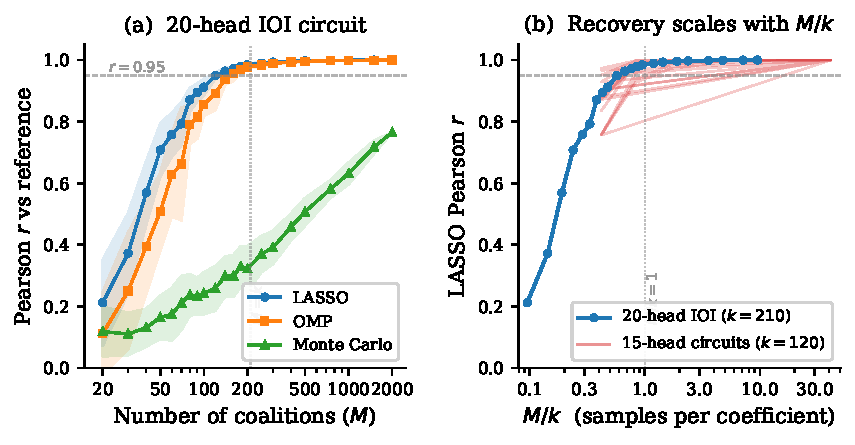
\includegraphics[width=0.95\linewidth]{sparse_walsh_recovery.pdf}
  \end{center}

  \vspace{4mm}
  {\small
  \begin{tabular}{lcc}
    \toprule
    \textbf{Method} & $M = 140$ & $M = 500$ \\
    \midrule
    LASSO    & $0.96 \pm 0.01$ & $0.99 \pm 0.00$ \\
    OMP      & $0.91 \pm 0.04$ & $0.98 \pm 0.01$ \\
    Monte Carlo & $0.78 \pm 0.03$ & $0.91 \pm 0.01$ \\
    \bottomrule
  \end{tabular}
  }

  \vspace{4mm}
  Recovery correlation ($r$) between sparse estimate and ground truth
  from exhaustive sweep. LASSO dominates at low $M$.
}

\end{columns}

% ════════════════════════════════════════════════════════
% ROW 2
% ════════════════════════════════════════════════════════
\begin{columns}
\column{0.50}

\block{Energy Spectrum Across Six Tasks}{
  \begin{center}
  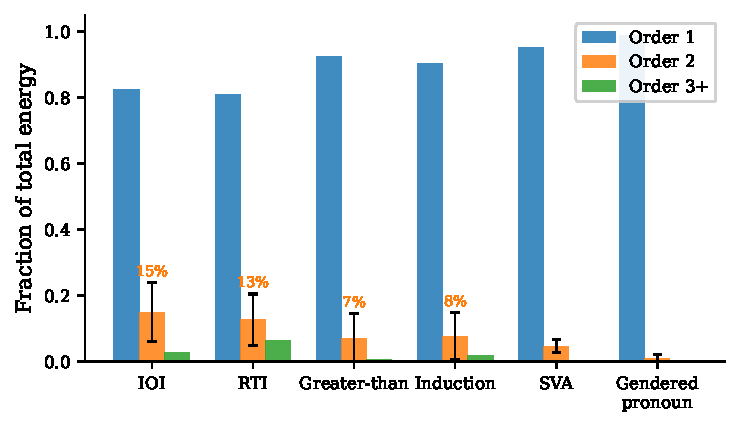
\includegraphics[width=0.70\linewidth]{energy_spectrum.pdf}
  \end{center}

  \vspace{4mm}
  {\small
  \begin{tabular}{lccc}
    \toprule
    \textbf{Task} & \textbf{Order 1} & \textbf{Order 2} & \textbf{Order 3+} \\
    \midrule
    IOI              & 0.82 & 0.15 & 0.03 \\
    RTI              & 0.81 & 0.13 & 0.06 \\
    Greater-than     & 0.92 & 0.07 & 0.01 \\
    Induction        & 0.90 & 0.08 & 0.02 \\
    SVA              & 0.95 & 0.05 & 0.00 \\
    Gendered pronoun & 0.99 & 0.01 & 0.00 \\
    \midrule
    Random           & 0.92 & 0.06 & 0.02 \\
    \bottomrule
  \end{tabular}
  }

  \vspace{4mm}
  60 sweeps across 6 tasks in GPT-2 small.
  Tasks requiring coordinated attention routing (IOI, RTI) carry
  13--15\% pairwise energy. Random head sets carry ${\sim}6\%$,
  confirming that interaction structure reflects functional coupling.
}

\column{0.50}

\block{Discovery Methods Disagree}{
  \begin{center}
  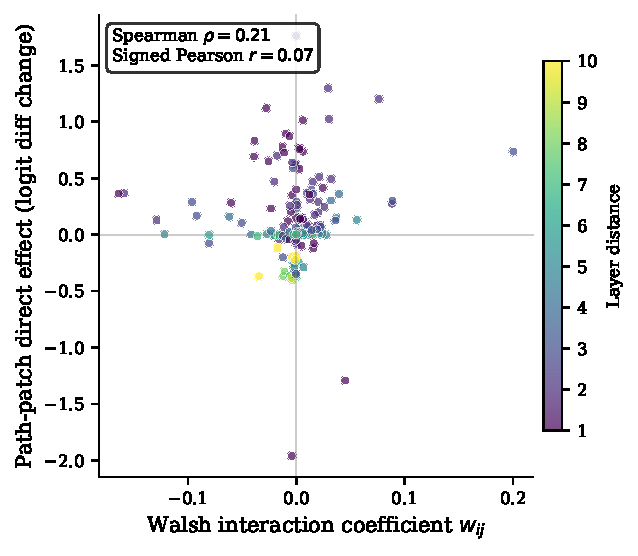
\includegraphics[width=0.65\linewidth]{path_patching_scatter.pdf}
  \end{center}

  \vspace{4mm}
  {\small
  \begin{tabular}{lcc}
    \toprule
    \textbf{Comparison} & \textbf{Spearman} $\rho$ & \textbf{Pearson} $r$ \\
    \midrule
    Walsh vs EAP-IG          & 0.58 & 0.73 \\
    Walsh vs path patching   & 0.21 & 0.07 \\
    \bottomrule
  \end{tabular}
  }

  \vspace{4mm}
  EAP-IG captures moderate interaction structure ($\rho = 0.58$).
  Path patching is \textbf{nearly orthogonal} ($r = 0.07$): its
  top-ranked pair (L10H7$\to$L11H1) ranks 42nd by Walsh.

  \vspace{6mm}
  \textbf{Weight geometry predicts nothing.} Cross-validated $R^2 < 0$
  across all 30 conditions (zero, mean, resample ablation $\times$
  10 geometric primitives). 32\% of pairwise geometric predictions
  have the wrong sign.
}

\end{columns}

% ════════════════════════════════════════════════════════
% ROW 3
% ════════════════════════════════════════════════════════
\begin{columns}
\column{0.50}

\block{What the Interactions Contain: Complementation Test}{
  \textbf{S-inhibition heads and negative name movers merge into one
  functional unit} in 1000/1000 bootstrap resamples (ARI = 0.571 against
  published IOI taxonomy). The merge holds across ablation methods,
  circuit selection methods, and linkage criteria.

  \vspace{6mm}
  \begin{center}
  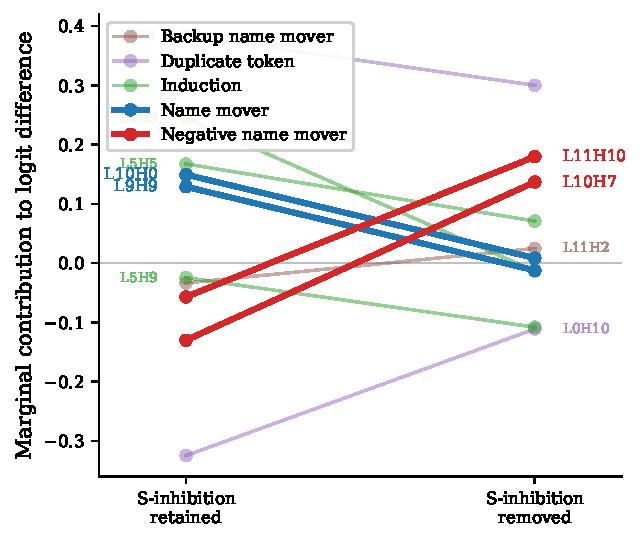
\includegraphics[width=0.70\linewidth]{conditional_marginal.pdf}
  \end{center}

  \vspace{4mm}
  Negative name movers \textbf{invert sign} when S-inhibition is
  removed: L10H7 goes from $-0.130$ to $+0.137$, L11H10 from $-0.057$
  to $+0.180$ (both flip in 1000/1000 draws). Name movers decay toward
  zero without inverting.

  \vspace{4mm}
  \textbf{An additive summary reports negative name movers as harmful.
  Their actual effect depends on S-inhibition state.}
}

\column{0.50}

\block{Walsh-Ranked Circuits Are Faithful (MIB)}{
  \begin{center}
  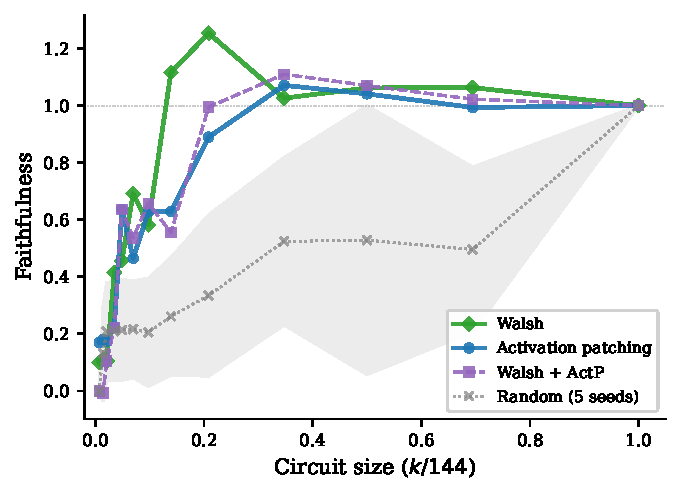
\includegraphics[width=0.70\linewidth]{mib_faithfulness_curves.pdf}
  \end{center}

  \vspace{4mm}
  {\small
  \begin{tabular}{lcc}
    \toprule
    \textbf{Method} & \textbf{CPR} $\uparrow$ & \textbf{CMD} $\downarrow$ \\
    \midrule
    Walsh                       & 0.996 & 0.100 \\
    Activation patching         & 0.937 & 0.095 \\
    Walsh + activation patching & 0.956 & 0.104 \\
    Random                      & $0.608 \pm 0.194$ & $0.402 \pm 0.180$ \\
    \bottomrule
  \end{tabular}
  }

  \vspace{4mm}
  Walsh reaches $f > 1.0$ at $k = 20$ heads (14\% of model), where
  activation patching is at $f = 0.63$. All 144 heads in GPT-2 small
  ranked; 16 of top 20 overlap between methods. Combining adds noise
  rather than complementary information.

  \vspace{8mm}
  \begin{center}
  {\large\textbf{Takeaway}}

  \vspace{4mm}
  A head's measured contribution is a property of the head\\
  together with the background it was measured against.\\
  Reporting it as a property of the head alone is safe only\\
  when the order-2 terms coupling it to the rest of the\\
  circuit are small. Those terms are measurable.

  \vspace{6mm}
  \texttt{elliot@elliottower.ai}
  \end{center}
}

\end{columns}

\end{document}
